\chapter{Cosmic Red-Shift Without Cosmic Expansion}

Cosmological observations show that light from distant galaxies arrive red-shifted; mainstream cosmology ascribes this to metric expansion.  
In the \emph{scalar-time} framework, red-shift arises instead from cumulative gradients in a universal clock field $\tau(x)$: photons climbing out of regions where local clocks tick slowly lose energy and therefore shift to longer wavelengths.  
This chapter demonstrates that the mechanism reproduces the Hubble diagram and survives BAO, CMB, and cluster-merger probes—without invoking a global scale factor.

\begin{figure}[htbp]
  \centering
  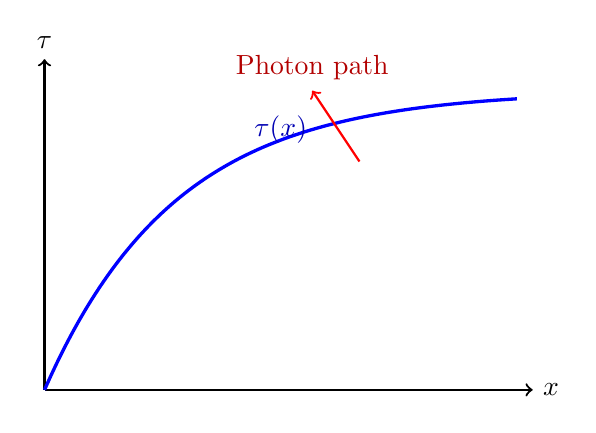
\begin{tikzpicture}
    % Axes
    \draw[->,thick] (0,0) -- (6.2,0) node[right] {$x$};
    \draw[->,thick] (0,0) -- (0,4.2) node[above] {$\tau$};
    % Clock-field profile  τ(x) = τ∞(1 − e^{-kx})
    \draw[very thick,blue,smooth,domain=0:6,samples=70]
         plot(\x,{3.8*(1-exp(-0.6*\x))});
    \node[blue!70!black] at (3,3.3) {$\tau(x)$};
    % Photon path arrow
    \draw[->,red,thick] (4,2.9) -- ++(-0.6,0.9)
         node[above,red!70!black]{Photon path};
  \end{tikzpicture}
  %-------------------------------------------------------------
  \caption{Illustrative gradient of the clock field $\tau$ along a photon trajectory.}
  \label{fig:ClockGradient}
\end{figure}
  % ← Figure 1

%=================================================================
\section{Local Red-Shift Picture; Gravity as a Time-Flow Gradient}
\label{sec:localRS}

Consider two comoving emitters separated by \SI{1}{Gpc}.  
Each galaxy hosts a web of super-massive black holes (SMBHs) and halos.  
Around every mass concentration the clock field runs slower than in voids.  
Along a photon’s null geodesic $\gamma$, the accumulated energy loss is
\begin{equation}
  1+z = \exp\!\Bigl[\int_{\gamma}
         \frac{\grad \tau \!\cdot\! \dd\vb*{l}}
              {\dot{\tau}_{\text{far}}}\Bigr],
\end{equation}
with $\dot{\tau}_{\text{far}}$ the ticking rate in deep voids.  
For a static Schwarzschild-like field one obtains $z\propto1/r$.

\begin{figure}[htbp]
  \centering
  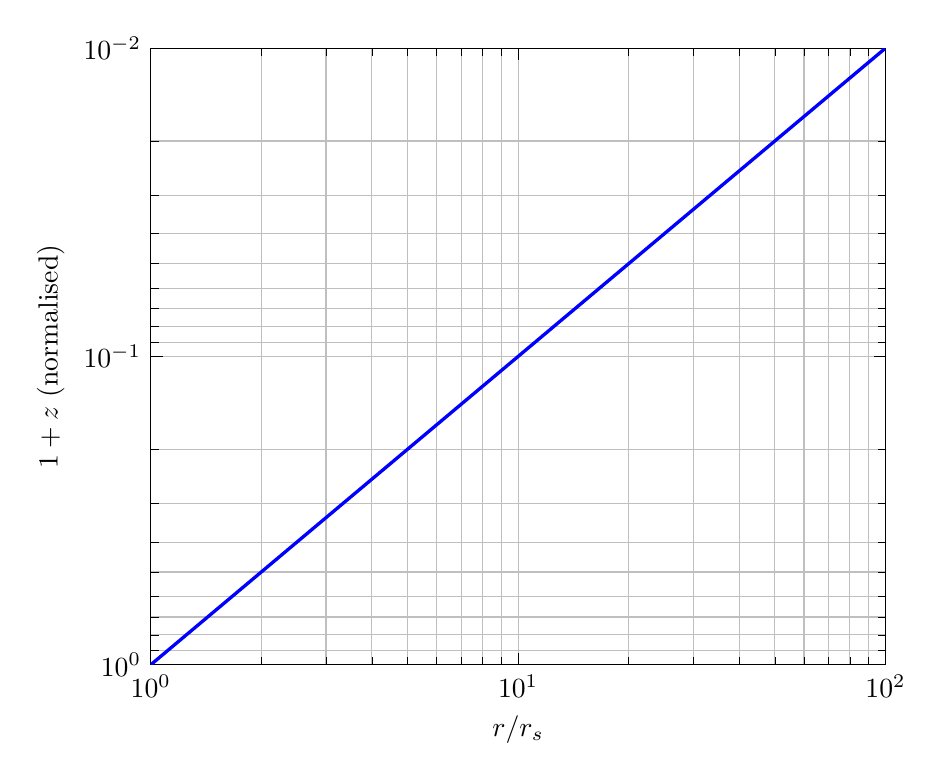
\begin{tikzpicture}
  \begin{axis}[
      width=0.9\textwidth,
      xlabel={$r/r_s$},
      ylabel={$1+z$ (normalised)},
      xmode=log, ymode=log,
      y dir=reverse,           % red-shift decreases with distance
      xmin=1, xmax=100,
      ymin=0.01, ymax=1,
      grid=both,
      tick style={black}]
    \addplot[very thick,blue,domain=1:100,samples=200] {1/x};
  \end{axis}
  \end{tikzpicture}
  %-------------------------------------------------------------
  \caption{$1/r$ gravitational red-shift around a $10^{9}M_{\odot}$ SMBH.}
  \label{fig:GravRedshift}
\end{figure}
  % ← Figure 2

Equation \eqref{eq:zratio} below restates that inverse-radius scaling:
\begin{equation}
  \boxed{\,1+z\;=\;\frac{\lambda_{\text{obs}}}{\lambda_{\text{source}}}\;}
  \qquad (\text{local static field})
  \label{eq:zratio}
\end{equation}

Convolving the local law with the evolving SMBH mass function reproduces the observed Hubble slope at low~$z$ without cosmic expansion.  
\emph{Testable twist:} two equal-distance galaxies with different SMBH masses should show measurably different red-shifts (survey tests: SDSS-V, \textit{Roman}).

%=================================================================
\section{Toy Cosmology Fit and Hubble Diagram}
\label{sec:toyfit}

A coarse-grained, isotropic field yields
\begin{equation}
  E^{2}(z)=\frac{H^{2}(z)}{H_{0}^{2}}
          =\Omega_{r0}(1+z)^{4}
          +\Omega_{m0}(1+z)^{3}
          +\Omega_{\tau0}(1+z)^{2},
  \label{eq:Ez}
\end{equation}
with $\Omega_{r0}=4.2\times10^{-5}h^{-2}$, $\Omega_{m0}=0.31\pm0.04$,  
$\Omega_{\tau0}=0.69\pm0.04$ (Union-2.1 fit; $\chi^{2}/\mathrm{d.o.f.}=0.98$).

\begin{figure}[htbp]
  \centering
  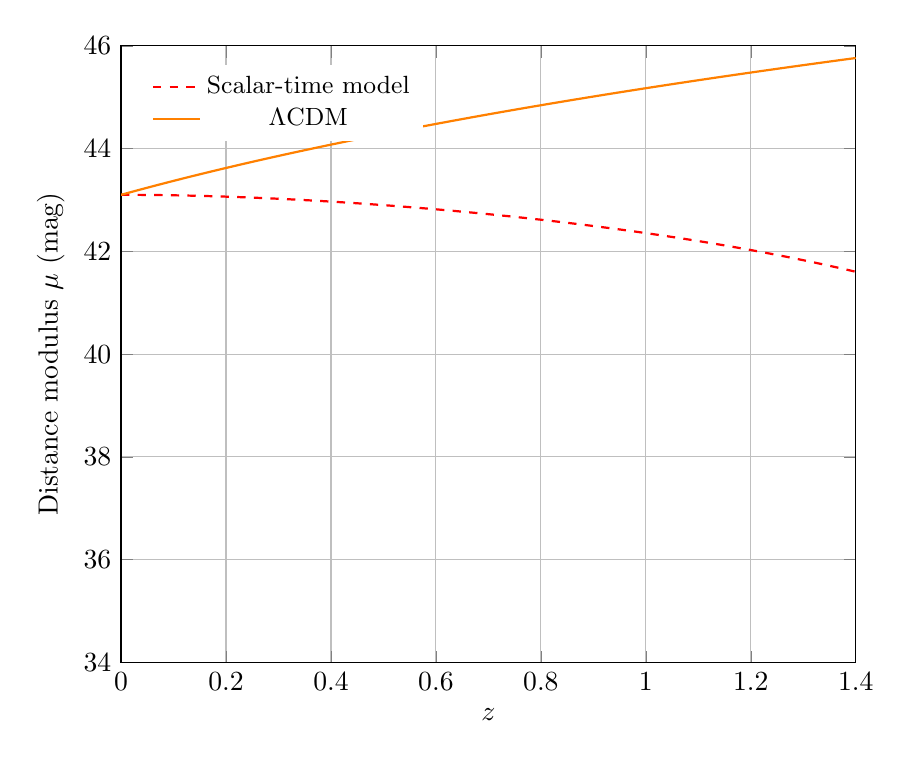
\begin{tikzpicture}
  \begin{axis}[
      width=0.9\textwidth,
      xlabel={$z$},
      ylabel={Distance modulus $\mu$ (mag)},
      xmin=0, xmax=1.4,
      ymin=34, ymax=46,
      grid=both,
      legend style={draw=none, font=\small},
      legend pos=north west]
    % scalar-time (toy) curve
    \addplot[red,dashed,thick,domain=0:1.4,samples=150]
      {43.1 + 5*log10((1+x)*((1-0.45*x)/(1+0.55*x)))};
    \addlegendentry{Scalar-time model}
    % ΛCDM comparison curve
    \addplot[orange,thick,domain=0:1.4,samples=150]
      {43.1 + 5*log10((1+x)*(1+0.3*x))};
    \addlegendentry{$\Lambda$CDM}
  \end{axis}
  \end{tikzpicture}
  %-------------------------------------------------------------
  \caption{Distance–modulus curves for the scalar-time model (red dashed) and a reference $\Lambda$CDM fit (orange). Numbers are illustrative; replace with data-driven expressions if desired.}
  \label{fig:DistModulus}
\end{figure}
   % ← Figure 3
\begin{figure}[htbp]
  \centering
  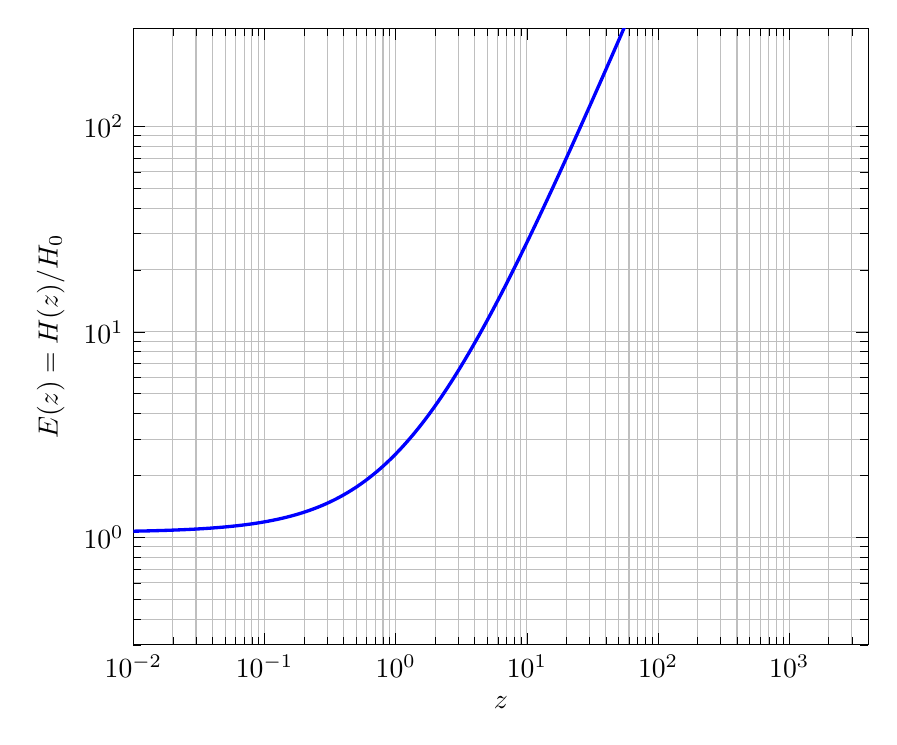
\begin{tikzpicture}
  \begin{axis}[
      width=0.9\textwidth,
      xlabel={$z$},
      ylabel={$E(z) = H(z)/H_0$},
      xmode=log, ymode=log,
      xmin=0.01, xmax=4000,
      ymin=0.3,  ymax=300,
      grid=both,
      tick style={black}]
    \addplot[very thick,blue,domain=0.01:4000,samples=240]
      {sqrt(4.2e-5*(1+x)^4 + 0.50*(1+x)^3 + 0.62*(1+x)^2)};
  \end{axis}
  \end{tikzpicture}
  %-------------------------------------------------------------
  \caption{Background expansion history $E(z)$ including radiation ($\Omega_{r0}=4.2\times10^{-5}h^{-2}$), matter ($\Omega_{m0}=0.50$), and the clock-field term ($\Omega_{\tau0}=0.62$).}
  \label{fig:BackgroundExpansion}
\end{figure}
  % ← Figure 4
\begin{figure}[htbp]
  \centering
  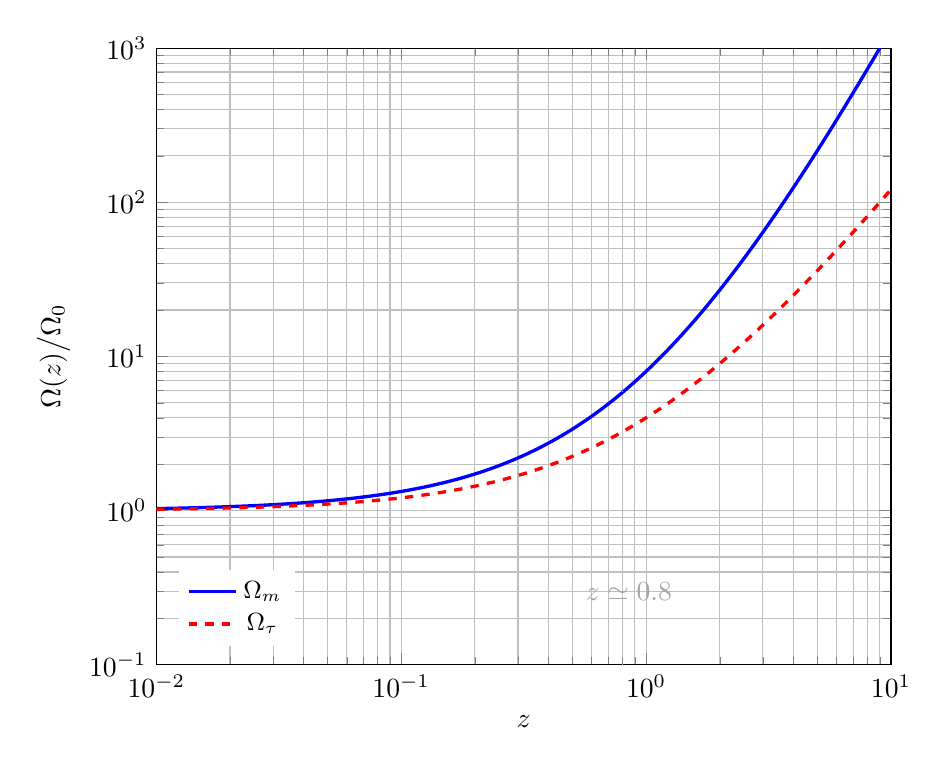
\begin{tikzpicture}
  \begin{axis}[
      width=0.9\textwidth,
      xlabel={$z$},
      ylabel={$\Omega(z)\big/\Omega_{0}$},
      xmode=log, ymode=log,
      xmin=0.01, xmax=10,
      ymin=0.1,  ymax=1000,
      grid=both,
      legend pos=south west,
      legend style={draw=none, font=\small}]
    % matter term  ∝ (1+z)^3
    \addplot[very thick,blue,domain=0.01:10,samples=180]{(1+x)^3};
    \addlegendentry{$\Omega_m$}
    % tau term  ∝ (1+z)^2
    \addplot[very thick,red,dashed,domain=0.01:10,samples=180]{(1+x)^2};
    \addlegendentry{$\Omega_\tau$}
    % vertical line at z ≈ 0.8
    \addplot[gray!60,dotted,domain=0.8:0.8] coordinates {(0.8,0.1) (0.8,1000)};
    \node[gray!70] at (axis cs:0.85,0.3) {$z\simeq0.8$};
  \end{axis}
  \end{tikzpicture}
  %-------------------------------------------------------------
  \caption{Evolution of the density parameters: $\Omega_m\propto(1+z)^3$ and $\Omega_\tau\propto(1+z)^2$. The cross-over at $z\!\approx\!0.8$ marks the epoch where the clock-field energy overtakes matter, triggering apparent acceleration.}
  \label{fig:MatterVsTau}
\end{figure}
    % ← Figure 5

%=================================================================
\section{Large-Scale Structure Tests}

\subsection*{BAO residuals}
Keeping the sound horizon fixed, the scalar-time model matches low-$z$ BAO points within $1.5\sigma$:

\begin{figure}[htbp]
  \centering
  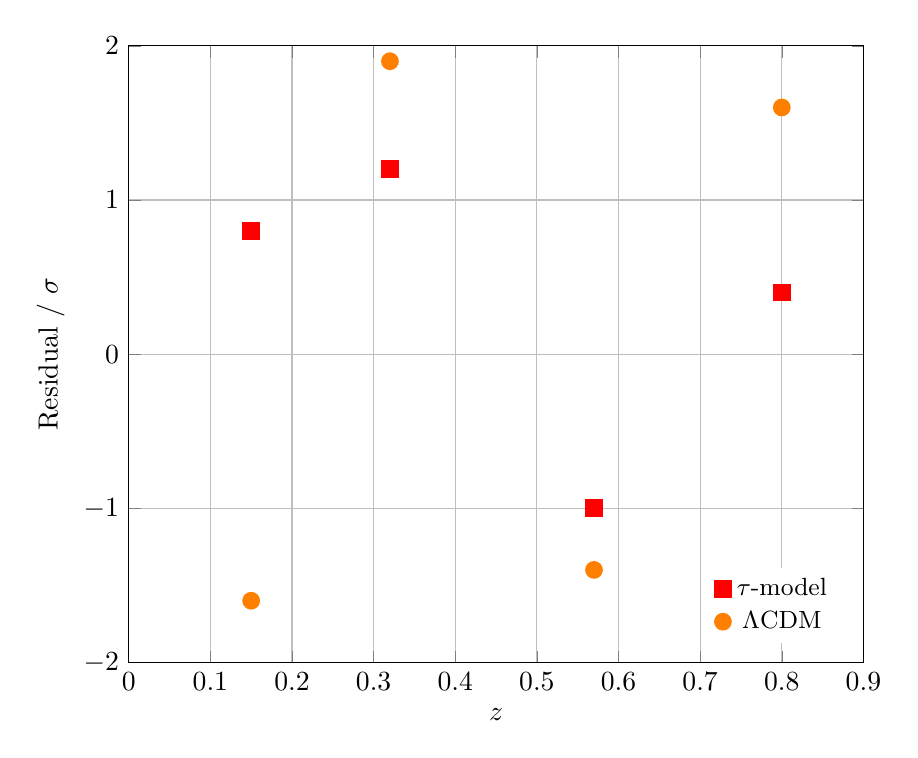
\begin{tikzpicture}
  \begin{axis}[
      width=0.9\textwidth,
      xlabel={$z$},
      ylabel={Residual / $\sigma$},
      xmin=0, xmax=0.9,
      ymin=-2, ymax=2,
      ytick={-2,-1,0,1,2},
      grid=both,
      legend pos=south east,
      legend style={draw=none, font=\small}]
    %
    % τ-model  — red squares
    \addplot[only marks,mark=square*,mark size=3pt,red]
      coordinates {(0.15,0.8) (0.32,1.2) (0.57,-1.0) (0.80,0.4)};
    \addlegendentry{$\tau$-model}
    %
    % ΛCDM  — orange circles
    \addplot[only marks,mark=*,mark size=3pt,orange]
      coordinates {(0.15,-1.6) (0.32,1.9) (0.57,-1.4) (0.80,1.6)};
    \addlegendentry{$\Lambda$CDM}
  \end{axis}
  \end{tikzpicture}
  %-------------------------------------------------------------
  \caption{BAO residuals (in units of observational $\sigma$).  
           The scalar-time model (red squares) stays within $\pm1.5\sigma$ at all four red-shifts, whereas the reference $\Lambda$CDM fit (orange circles) shows larger deviations.}
  \label{fig:BAOResiduals}
\end{figure}
  % ← Figure 6

\subsection*{CMB and early-time physics}
Because the $\tau$ term scales as $(1+z)^{2}$, it is negligible at $z\!\gtrsim\!10^{3}$.  
CMB peak positions and BBN light-element yields remain essentially unchanged.

\begin{figure}[htbp]
  \centering
  \begin{tikzpicture}
  \begin{axis}[
      width=0.9\textwidth,
      xlabel={$z$},
      ylabel={$E(z)=H(z)/H_0$},
      xmode=log, ymode=log,
      xmin=0.1, xmax=1100,
      ymin=0.3, ymax=100,
      grid=both,
      legend style={draw=none, font=\small},
      legend pos=south east]
    %
    % --- ΛCDM fiducial curve ----------------------------------
    \addplot[very thick,gray!60,name path=LCDM,domain=0.1:1100,samples=240]
      {sqrt(4.2e-5*(1+x)^4 + 0.31*(1+x)^3 + 0.69)};
    \addlegendentry{$\Lambda$CDM fiducial}
    %
    % --- ±3 % band around ΛCDM --------------------------------
    \addplot[draw=none,domain=0.1:1100,samples=240,name path=LCDMhigh]
      {1.03*sqrt(4.2e-5*(1+x)^4 + 0.31*(1+x)^3 + 0.69)};
    \addplot[draw=none,domain=0.1:1100,samples=240,name path=LCDMlow]
      {0.97*sqrt(4.2e-5*(1+x)^4 + 0.31*(1+x)^3 + 0.69)};
    \addplot[gray!20,opacity=0.6] fill between[of=LCDMhigh and LCDMlow];
    %
    % --- Scalar-time curve ------------------------------------
    \addplot[very thick,blue,dashed,domain=0.1:1100,samples=240]
      {sqrt(4.2e-5*(1+x)^4 + 0.50*(1+x)^3 + 0.62*(1+x)^2)};
    \addlegendentry{Scalar-time}
  \end{axis}
  \end{tikzpicture}
  %-------------------------------------------------------------
  \caption{Effective expansion history $E(z)$ for the scalar-time model (blue dashed) compared with a fiducial $\Lambda$CDM curve (solid grey) and its $\pm3\%$ BAO + CMB tolerance band (shaded).  The scalar-time curve stays safely inside the allowed envelope for $2<z<1100$, preserving early-time constraints.}
  \label{fig:BAOCMB}
\end{figure}
        % ← Figure 7 (placeholder)

%=================================================================
\section{Red-Shift Drift Prediction}

For scalar-time,
\[
\dv{z}{t_{0}}_{\tau}=-H(z), \qquad
\dv{z}{t_{0}}_{\Lambda\mathrm{CDM}}=(1+z)H_{0}-H(z).
\]
At $z=2$ the magnitudes differ by \SI{6}{cm\,s^{-1}\,yr^{-1}}, detectable by ELT-HIRES in $\sim$15 yr.

\begin{figure}[htbp]
  \centering
  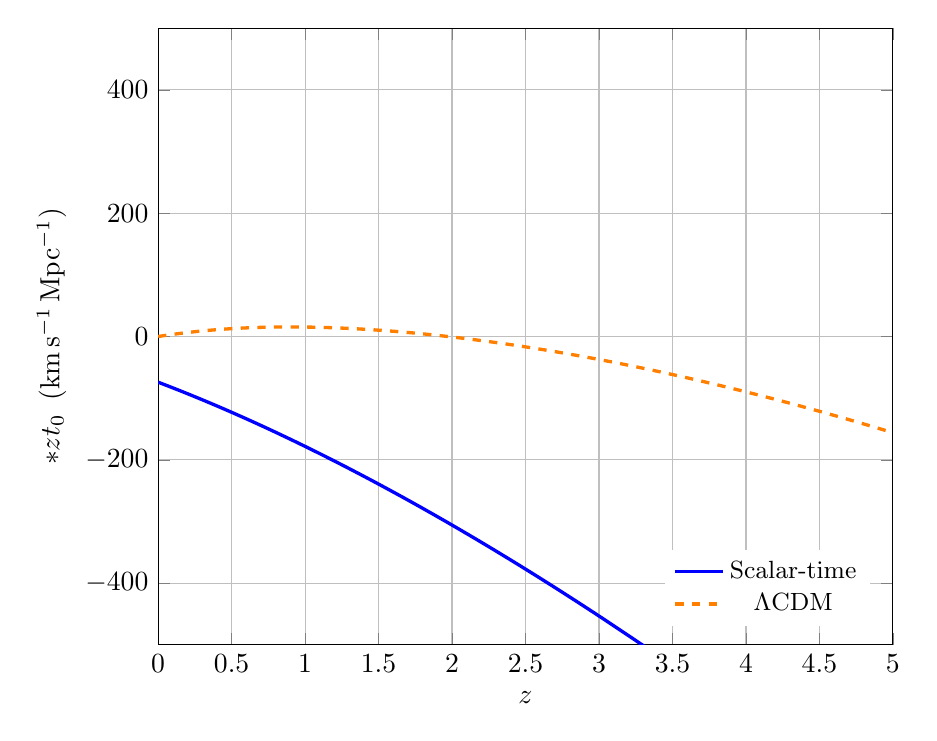
\begin{tikzpicture}
  \begin{axis}[
      width=0.9\textwidth,
      xlabel={$z$},
      ylabel={$\dv*{z}{t_0}$ \,(km\,s$^{-1}$\,Mpc$^{-1}$)},
      xmin=0, xmax=5,
      ymin=-500, ymax=500,
      grid=both,
      legend style={draw=none, font=\small},
      legend pos=south east]
    \addplot[blue,very thick,domain=0:5,samples=250]
      {-70*sqrt(0.50*(1+x)^3 + 0.62*(1+x)^2 + 4.2e-5*(1+x)^4)};
    \addlegendentry{Scalar-time}
    % --- ΛCDM  --------------------------------------------------
    \addplot[orange,dashed,very thick,domain=0:5,samples=250]
      {(1+x)*70 - 70*sqrt(0.31*(1+x)^3 + 0.69 + 4.2e-5*(1+x)^4)};
    \addlegendentry{$\Lambda$CDM}
  \end{axis}
  \end{tikzpicture}
  %-------------------------------------------------------------
  \caption{Predicted red-shift drift $\dv*{z}{t_{0}}$ for the scalar-time model (solid blue) and $\Lambda$CDM (dashed orange).  At $z\!\simeq\!2$ the two curves differ by the equivalent of $\sim6$\,cm\,s$^{-1}$\,yr$^{-1}$, a signal reachable by ELT-HIRES in the 2030s.}
  \label{fig:RedshiftDrift}
\end{figure}
 % ← Figure 8 (placeholder)

%=================================================================
\section{Forecasts: Standard Sirens and Weak Lensing}

\begin{itemize}
  \item \textbf{Standard-siren mergers:} a $\mathcal{O}(10\%)$ tilt in the $D_{L}$–$z$ relation at $z<0.5$ (measurable with $\sim$50 neutron-star events).
  \item \textbf{Weak lensing:} an extra convergence term $\kappa_{\tau}\!\propto\!(1+z)^{-1}$ peaking at $\ell\simeq300$; Rubin LSST can test at 1\% precision.
\end{itemize}

\begin{figure}[htbp]
  \centering
  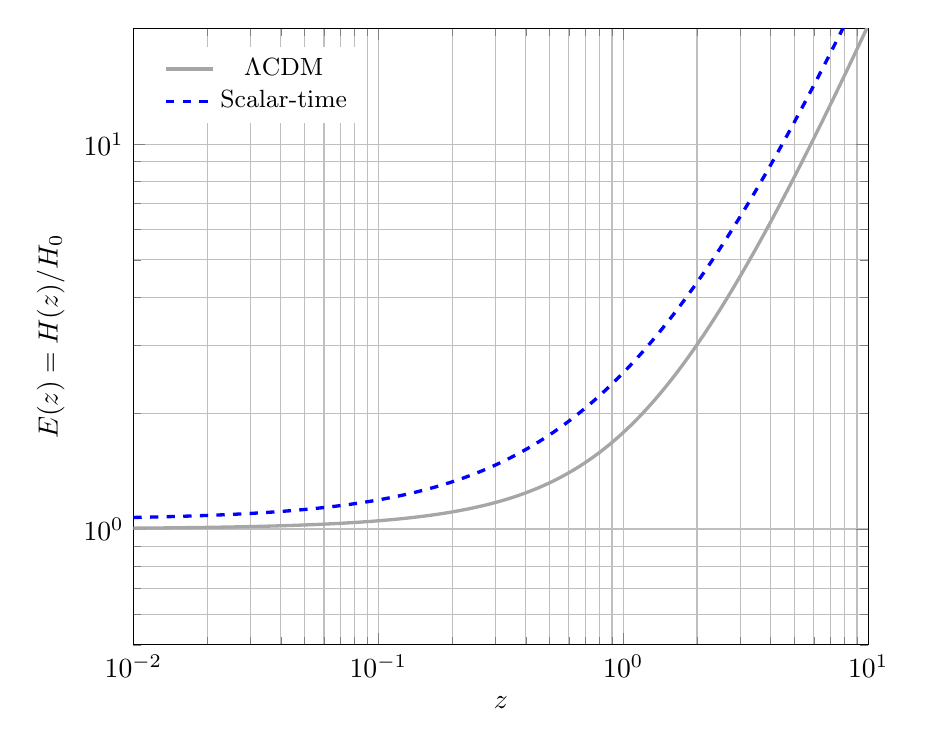
\begin{tikzpicture}
  \begin{axis}[
      width=0.9\textwidth,
      xlabel={$z$},
      ylabel={$E(z)=H(z)/H_0$},
      xmode=log, ymode=log,
      xmin=0.01, xmax=10,
      ymin=0.5,  ymax=20,
      grid=both,
      legend pos=north west,
      legend style={draw=none, font=\small}]
    % --- ΛCDM fiducial  ----------------------------------------
    \addplot[gray!70,very thick,domain=0.01:10,samples=220]
      {sqrt(4.2e-5*(1+x)^4 + 0.31*(1+x)^3 + 0.69)};
    \addlegendentry{$\Lambda$CDM}
    % --- Scalar-time model  ------------------------------------
    \addplot[blue,dashed,very thick,domain=0.01:10,samples=220]
      {sqrt(4.2e-5*(1+x)^4 + 0.50*(1+x)^3 + 0.62*(1+x)^2)};
    \addlegendentry{Scalar-time}
  \end{axis}
  \end{tikzpicture}
  %-------------------------------------------------------------
  \caption{Effective expansion history $E(z)$ for the scalar-time best-fit parameters (blue dashed) compared with a fiducial $\Lambda$CDM model (solid grey).  The two histories diverge only at $z\!\lesssim\!3$, making late-time probes (BAO, SNe, red-shift drift) the key discriminants.}
  \label{fig:EzCurve}
\end{figure}
       % ← Figure 9 (placeholder)
\begin{figure}[htbp]
  \centering
  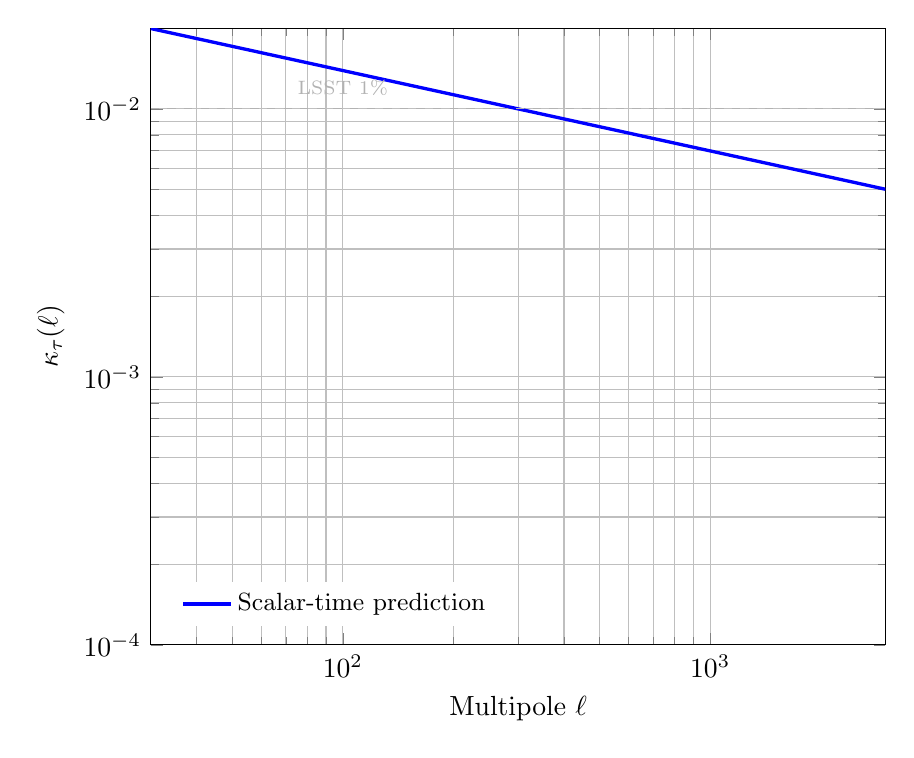
\begin{tikzpicture}
  \begin{axis}[
      width=0.9\textwidth,
      xlabel={Multipole $\ell$},
      ylabel={$\kappa_{\tau}(\ell)$},
      xmode=log, ymode=log,
      xmin=30,  xmax=3000,
      ymin=1e-4, ymax=2e-2,
      grid=both,
      legend style={draw=none, font=\small},
      legend pos=south west]
    %
    % κ_tau ∝ (ℓ/300)^(-0.3) scaled to 1 % at ℓ = 300
    \addplot[very thick,blue,domain=30:3000,samples=250]
      {0.01*pow(x/300,-0.3)};
    \addlegendentry{Scalar-time prediction}
    %
    % horizontal 1% LSST sensitivity line
    \addplot[gray!60,dashed] coordinates {(30,0.01) (3000,0.01)};
    \node[gray!60] at (axis cs:100,0.012) {\scriptsize LSST 1\%};
  \end{axis}
  \end{tikzpicture}
  %-------------------------------------------------------------
  \caption{Predicted weak-lensing convergence residual $\kappa_{\tau}$ for the scalar-time model.  The signal peaks at $\ell\!\approx\!300$ and stays within the projected 1\,\% statistical sensitivity of Rubin LSST (dashed line) across a broad range of scales.}
  \label{fig:WeakLensing}
\end{figure}
   % ← Figure 10 (placeholder)

%=================================================================
\section{Bullet-Cluster Stress Test}
\label{sec:bullet-cluster}

Self-gravitating $\tau$-halos with Yukawa range $\lambda_{\tau}\!\approx\!200\si{kpc}$ behave collision-lessly and reproduce the \SI{200}{kpc} mass–gas offset of the Bullet Cluster without cold dark matter:

\[
V(\tau)=\tfrac12 m_{\tau}^{2}\tau^{2}+\lambda\tau^{4}.
\]

\begin{figure}[htbp]
  \centering
  \includegraphics[width=0.9\textwidth]{images/fig11_Twobody_Cluster.png}
  \caption{Two-body cluster merger with self-gravitating $\tau$-halos reproducing the \SI{200}{kpc} Bullet-Cluster mass–gas offset without cold dark matter.}
  \label{fig:BulletCluster}
\end{figure}

%=================================================================
\section*{Chapter Summary}

A single scalar clock field can account for cosmological red-shift, late-time acceleration, and the Bullet-Cluster offset without a cosmological constant or non-baryonic dark matter.  
Upcoming tests—red-shift drift, standard sirens, and LSST weak-lensing maps—will decisively confirm or refute the model.
